
\section{Address Spaces}

The full accessible Program memory can be accessed by \verb|PEEK|/\verb|POKE|, 
\verb|LPEEK|/\verb|LPOKE|, \verb|DPEEK|/\verb|DPOKE|. Be careful. You can
manipulate all symbols of the interpreter and or dynamically linked libraries
and your program. Address spaces belonging to other programs which are not
shared memory blocks can not be accessed. You will get a segmentation fault on
trying this.

\section{Graphics: Drawing and Painting}

A graphics window will be automatically opened when the first graphic command
appears in your program. Without using any graphic commands no X11-Server is
needed at all and your programs also runs under a text console or as a daemon
or as CGI scripts. But if you want to draw anything with e.g. \verb|LINE|,
\verb|CIRCLE| or \verb|BOX|, control the MOUSE pointer, the keyboard or use
the graphical user interface with e.g. \verb|ALERT| or \verb|MENU|, a graphic
window will open with the default geometry \verb|640x400|. All graphic output
can be done in full color which can be set with the \verb|GET_COLOR()| and the
\verb|COLOR| statements. Moreover, there can be up to 16 different graphic
windows opened at a time. Please note that all graphics is displayed after a
\verb|SHOWPAGE| command only. This allows fast animations.

To allow for animated bitmap graphics and icons, X11-Basic offers the commands
\verb|GET| and \verb|PUT|, which retrieve rectangular regions from the
graphics-window into a string or put back bitmap graphics data from the 
string to the graphics screen or window. The file format used with 
\verb|PUT| is a standard .BMP bitmap, so also externally created icons can be
used. Transparency and alpha channels are supported.


\section{Reading from and Writing to Files}

Before you may read from or write to a file, you need to open it; once you are
done, you should close it. Each open file is designated by a simple number,
which might be stored within a variable and must be supplied to the \verb|PRINT|
and \verb|INPUT| commands if you want to access the file. 

If you need more control, you may consider reading and writing one byte at a
time, using the multi-purpose commands \verb|INP()| and \verb|OUT|, or reading
the whole file as a binary block with \verb|BLOAD|.

\section{Internet and bluetooth connections, special files and sockets}

X11-Basic allows to connect a program to another program on a different (or the
same) host computer via standard internet or bluetooth protocols or pipes. 

Basically there are two methods of connections to other computers on a network: 
A stream based connections (well known is the TCP/IP protocol for internet
connections) and a connectionless, unreliable datagram packet service (UDP, in
case of internet connections, and e.g. L2CAP for bluetooth). 

Another method of passing data between two applications on the same computer is
using so-called pipes. Pipes are special files which are created in the local
filesystem. 

\subsection{Local inter process communication: Pipes}

A pipe is a unidirectional data channel that can be used for interprocess 
communication. The UNIX kernel usually supports this mechanism. The pipe can be
used to send information or data from one process to another. Here is a little
example progam you can use to play with it:

\begin{mdframed}[hidealllines=true,backgroundcolor=blue!20]
{\footnotesize
\begin{verbatim}
PIPE #1,#2
a=FORK()
IF a=0    ! Child instance
  GPRINT "Hi, I am Child !",b
  DO
    SHOWPAGE
    LINEINPUT #1,t$
    GPRINT t$
  LOOP
  ' This instance never ends ...
ELSE IF a=-1  
  PRINT "ERROR, fork() failed !"
  QUIT
ELSE      ! parent instance
  DO
    DUMP
    ALERT 1,"Hi, I am Parent. Child PID="+str$(a),1," OK | Kill Child ! ",b
    DUMP
    PRINt #2,SYSTEM$("date")
    FLUSH #2
    IF b=2
      SYSTEM "kill "+str$(a)
      ALERT 1,"Child PID="+str$(a)+" killed !",1," OK ",b
      QUIT
    ENDIF
  LOOP
ENDIF
QUIT
\end{verbatim} }
\end{mdframed}

Instad of with pipes, the interprocess communication can also be done using a
shared memory segment. X11-Basic also supports commands for creating and
accessing such shared memory segments.


\subsection{World-Wide communication: Sockets}

Most inter-process communication uses the client server model. These terms refer
to the two processes which will be communicating with each other. One of the two
processes, the client, connects to the other process, the server, typically to
make a request for information. A good analogy is a person who makes a phone
call to another person.

Notice that the client needs to know of the existence of and the address of the
server, but the server does not need to know the address of (or even the
existence of) the client prior to the connection being established. Notice also
that once a connection is established, both sides can send and receive
information.

When a socket is created, the program has to specify the address domain and the
socket type. Two processes can communicate with each other only if their sockets
are of the same type and in the same domain. There are two widely used address
domains, the (local) Unix domain, in which two processes which share a common
file system communicate, and the Internet domain, in which two processes running
on any two hosts on the Internet communicate. Each of these has its own address
format. Another domain to be mentioned is the bluetooth domain for short range
radio connections. It works similar to the internet connections, but uses its
own address space.

The address of a socket in the Unix domain is a character string which is
basically an entry in the file system. It can be acced from there like a file. 
In X11-Basic the normal file i/o commands can be used. 

The address of a socket in the Internet domain consists of the Internet address
of the host machine (every computer on the Internet has a unique 32 bit address,
often referred to as its IP address or the bluetooth id, if we are takling about
bluetooth connections). In addition, each socket needs a port number on that
host. Port numbers are 16 bit unsigned integers. The lower numbers are reserved
in the internet for standard services. For example, the port number for the FTP
server is 21. It is important that standard services be at the same port on all
computers so that clients will know their addresses. However, port numbers above
2000 are generally available.

\paragraph{Socket Types}

There are two widely used socket types, stream sockets, and datagram sockets.
Stream sockets treat communications as a continuous stream of characters, while
datagram sockets have to read entire messages at once. Each uses its own
communications protocol. Stream sockets for internet connections use TCP
(Transmission Control Protocol), which is a reliable, stream oriented protocol,
and datagram sockets use UDP (Unix Datagram Protocol), which is unreliable and
message oriented.

The same applies for bluetooth connections, stream sockets use the so-called
RFCOMM protocol and datagram sockets use the L2CAP protocol.

Sockets in X11-Basic can be crated with the OPEN command.

\paragraph{TCP/IP}

Transmission Control Protocol (TCP) provides a reliable byte-stream transfer
service between two endpoints on an internet. TCP depends on IP to move packets
around the network on its behalf. IP is inherently unreliable, so TCP protects
against data loss, data corruption, packet reordering and data duplication by
adding checksums and sequence numbers to transmitted data and, on the receiving
side, sending back packets that acknowledge the receipt of data.

Before sending data across the network, TCP establishes a connection with the
destination via an exchange of management packets. The connection is destroyed,
again via an exchange of management packets, when the application that was using
TCP indicates that no more data will be transferred. 

TCP has a multi-stage flow-control mechanism which continuously adjusts the
sender's data rate in an attempt to achieve maximum data throughput while
avoiding congestion and subsequent packet losses in the network. It also
attempts to make the best use of network resources by packing as much data as
possible into a single IP packet.

The system calls for establishing a connection are somewhat different for the
client and the server, but both involve the basic construct of a socket. A
socket is one end of an inter-process communication channel. The two processes
each establish their own socket.

The steps involved in establishing a socket on the client side are as follows:

\begin{enumerate}
   \item Create a socket with the OPEN command providing a port number
\begin{mdframed}[hidealllines=true,backgroundcolor=blue!20]
\begin{verbatim}
  OPEN "US",#1,"client",5000
\end{verbatim}\end{mdframed}
   \item Connect the socket to the address of the server using the CONNECT command
\begin{mdframed}[hidealllines=true,backgroundcolor=blue!20]
\begin{verbatim}
  CONNECT #1,"ptbtime1.ptb.de",13
\end{verbatim}\end{mdframed}
\item Instead of using Steps 1 and 2, you can alternatively use the combined
 command:
\begin{mdframed}[hidealllines=true,backgroundcolor=blue!20]
\begin{verbatim}
  OPEN "UC",#2,"ptbtime1.ptb.de",13
\end{verbatim}\end{mdframed}
   \item Send and receive data. There are a number of ways to do this, but the 
   simplest is to use the PRINT, SEND, WRITE, READ, RECEIVE INPUT commands. 
\begin{mdframed}[hidealllines=true,backgroundcolor=blue!20]
\begin{verbatim}
  PRINT #2,"GET /index.html"
  FLUSH #2
  WHILE INP?(#2)
    LINEINPUT #2,t$
    PRINT "got: ";t$
  WEND
\end{verbatim}\end{mdframed}
 \item close the connection with
\begin{mdframed}[hidealllines=true,backgroundcolor=blue!20]
\begin{verbatim}
 CLOSE #1
\end{verbatim}\end{mdframed}
\end{enumerate}

The steps involved in establishing a socket on the server side are as follows:

\begin{enumerate}
   \item Create a socket with the OPEN command and bind the socket to a port 
   number on the host machine.
\begin{mdframed}[hidealllines=true,backgroundcolor=blue!20]
\begin{verbatim}
  OPEN "US",#1,"server",5000
\end{verbatim}\end{mdframed}
   \item Listen for connections and
   \item Accept a connection with this other OPEN command, which opens 
   a connection to the connected client: 
\begin{mdframed}[hidealllines=true,backgroundcolor=blue!20]
\begin{verbatim}
  OPEN "UA",#2,"",1
\end{verbatim}\end{mdframed}
   This call typically blocks until a client connects with the server.
   \item Send and receive data on the accepted connection
\begin{mdframed}[hidealllines=true,backgroundcolor=blue!20]
\begin{verbatim}
  PRINT #2,"Welcome to X11-Basic test-server ..."
  FLUSH #2
  DO
    IF INP?(#2)
      LINEINPUT #2,t$
      PRINT "got: ";t$
    ENDIF
    EXIT IF t$="quit"
  LOOP
  PRINT #2,"goodbye..."
  FLUSH #2
\end{verbatim}\end{mdframed}
 \item close the established connection with
\begin{mdframed}[hidealllines=true,backgroundcolor=blue!20]
\begin{verbatim}
 CLOSE #2
\end{verbatim}\end{mdframed} and listen to the next connection (folow step 3) or 
 \item close the socket if not further needed.
\begin{mdframed}[hidealllines=true,backgroundcolor=blue!20]
\begin{verbatim}
 CLOSE #1
\end{verbatim}\end{mdframed}
\end{enumerate}

\paragraph{UDP}
 
User Datagram Protocol (UDP) provides an unreliable packetized data transfer
service between endpoints on a network. 

First, a socket has to be crated with the OPEN command:

\begin{mdframed}[hidealllines=true,backgroundcolor=blue!20]
\begin{verbatim}
  OPEN "UU",#1,"sender",5556
\end{verbatim}
\end{mdframed}

When a UDP socket is created, its local and remote addresses are
unspecified. Datagrams can be sent immediately using SEND with a valid
destination address and port as argument:
\begin{mdframed}[hidealllines=true,backgroundcolor=blue!20]
{\footnotesize\linespread{0.8}\begin{verbatim}
SEND #1,"This is my message",CVL(CHR$(131)+CHR$(195)+CHR$(15)+CHR$(200)),5000
\end{verbatim}}
\end{mdframed}
   
UDP uses the IPv4 address format, so a long integer has to be passed.

When CONNECT is called on the socket the default destination address is set and
datagrams can now be sent using SEND without specifying an destination address.
It is still possible to send to other destinations by passing an address to
SEND.

\begin{mdframed}[hidealllines=true,backgroundcolor=blue!20]
\begin{verbatim}
CONNECT #1,"localhost",5555
SEND #1,"This is my message"
\end{verbatim}
\end{mdframed}

All receive operations return only one packet.
       
\begin{mdframed}[hidealllines=true,backgroundcolor=blue!20]
\begin{verbatim}
IF INP?(#1)
  RECEIVE #1,t$,adr
  PRINT "Received Message: ";t$;" from ";HEX$(adr)
ENDIF
\end{verbatim}
\end{mdframed}

INP?(\#n) Returns the size of the next pending datagram in bytes, or 0 when no
datagram is pending.

The Socket should be closed when the connection is not going to be used any more:
\begin{mdframed}[hidealllines=true,backgroundcolor=blue!20]
\begin{verbatim}
CLOSE #1
\end{verbatim}
\end{mdframed}

UDP does not guarantee to actually deliver the data to the destination, nor does
it guarantee that data packets will be delivered to the destination in the order
in which they were sent by the source, nor does it guarantee that only one copy
of the data will be delivered to the destination. UDP does guarantee data
integrity, and it does this by adding a checksum to the data before
transmission. 

\section{Bluetooth connections}

Establishing a connection between two devices with a bluetooth adapter is
similar to the internet connections. Also here you can use a stream based
connection (using RFCOMM) or a datagram based one (using L2CAP).

The X11-Basic commands for doing so are also similar. The only noticable
difference is that instead of a IP address a bluetooth id need to be used and
there is no domain name system which can be asked for the address/id of a
device knowing its name. 

That means, if you want to connect to a bluetooth device, you need to know its
id before. The id consists of six bytes (instead of four in case of a IPV4
internet address). They are usually noted as a string of the format:
hh:hh:hh:hh:hh:hh with all 6 bytes in two-digit hex values separated by colons:
e.g. "78:F5:FD:15:4A:3A".

You can either hardcode the id in your program, or you can scan for visible
bluetooth devices. 

The scan can be done in X11-Basic with the FSFIRST\$() and FSNEXT\$() functions:

\begin{mdframed}[hidealllines=true,backgroundcolor=blue!20]
\begin{verbatim}
a$=FSFIRST$("","*","b")
WHILE LEN(a$)
  PRINT a$
  PRINT "Adress: ";WORD$(a$,1)
  PRINT "Name:   ";WORD$(a$,2)
  adr$=WORD$(a$,1)
  a$=FSNEXT$()
WEND
\end{verbatim}
\end{mdframed}

\paragraph{RFCOMM}

RFCOMM (Radio frequency communication) provides a simple reliable data stream to
the user, similar to TCP. 

Many Bluetooth applications use RFCOMM because of its widespread support and 
publicly available API on most operating systems. Additionally, applications
that used a serial port to communicate can be quickly ported to use RFCOMM.

As with TCP/IP establishing a connection via RFCOMM involves the basic construct
of a socket. The two processes (server and client) each establish their own
socket.

The steps involved in establishing a socket on the client side are as follows 
(assuming, that the bluetooth id you ant to connect to is in adr\$):


\begin{enumerate}
   \item Create a socket with the OPEN command providing a port number (TODO??)
%\begin{mdframed}[hidealllines=true,backgroundcolor=blue!20]
%\begin{verbatim}
%  OPEN "US",#1,"client",5000 ????????
%\end{verbatim}\end{mdframed}
   \item Connect the socket to the address of the server using the CONNECT command
%\begin{mdframed}[hidealllines=true,backgroundcolor=blue!20]
%\begin{verbatim}
%  CONNECT #1,adr$,13?????
%\end{verbatim}\end{mdframed}
\item Instead of using Steps 1 and 2, you can alternatively use the combined
 command:
%\begin{mdframed}[hidealllines=true,backgroundcolor=blue!20]
%\begin{verbatim}
%  OPEN "UB",#2,adr$,13  ?????
%\end{verbatim}\end{mdframed}
   \item Send and receive data. There are a number of ways to do this, but the 
   simplest is to use the PRINT, SEND, WRITE, READ, RECEIVE INPUT commands. 
\begin{mdframed}[hidealllines=true,backgroundcolor=blue!20]
\begin{verbatim}
  PRINT #2,"Hello"
  FLUSH #2
  WHILE INP?(#2)
    LINEINPUT #2,t$
    PRINT "got: ";t$
  WEND
\end{verbatim}\end{mdframed}
 \item close the connection with
\begin{mdframed}[hidealllines=true,backgroundcolor=blue!20]
\begin{verbatim}
 CLOSE #1
\end{verbatim}\end{mdframed}
\end{enumerate}

The steps involved in establishing a socket on the server side are as follows:

\begin{enumerate}
   \item Create a socket with the OPEN command and bind the socket to a port 
   number on the host machine. (TODO: port number ????)
%\begin{mdframed}[hidealllines=true,backgroundcolor=blue!20]
%\begin{verbatim}
%  OPEN "UZ",#1,"server",5000 ?????
%\end{verbatim}\end{mdframed}
   \item Listen for connections and
   \item Accept a connection with this other OPEN command, which opens 
   a connection to the connected client: 
\begin{mdframed}[hidealllines=true,backgroundcolor=blue!20]
\begin{verbatim}
  OPEN "UA",#2,"",1
\end{verbatim}\end{mdframed}
   This call typically blocks until a client connects with the server.
   \item Send and receive data on the accepted connection
\begin{mdframed}[hidealllines=true,backgroundcolor=blue!20]
\begin{verbatim}
  PRINT #2,"Welcome to X11-Basic test-server ..."
  FLUSH #2
  DO
    IF INP?(#2)
      LINEINPUT #2,t$
      PRINT "got: ";t$
    ENDIF
    EXIT IF t$="quit"
  LOOP
  PRINT #2,"goodbye..."
  FLUSH #2
\end{verbatim}\end{mdframed}
 \item close the established connection with
\begin{mdframed}[hidealllines=true,backgroundcolor=blue!20]
\begin{verbatim}
 CLOSE #2
\end{verbatim}\end{mdframed} and listen to the next connection (folow step 3) or 
 \item close the socket if not further needed.
\begin{mdframed}[hidealllines=true,backgroundcolor=blue!20]
\begin{verbatim}
 CLOSE #1
\end{verbatim}\end{mdframed}
\end{enumerate}


\paragraph{L2CAP}
(Logical link control and adaptation protocol)

First, a socket has to be crated with the OPEN command:

%\begin{mdframed}[hidealllines=true,backgroundcolor=blue!20]
%\begin{verbatim}
%  OPEN "UV oder L",#1,"sender",5556   ??????
%\end{verbatim}
%\end{mdframed}

When a L2CAP socket is created, its local and remote addresses are
unspecified. Datagrams can be sent immediately using SEND with a valid
destination address and port as argument:
%\begin{mdframed}[hidealllines=true,backgroundcolor=blue!20]
%{\footnotesize\linespread{0.8}\begin{verbatim}
%SEND #1,"This is my message",CVL(CHR$(131)+CHR$(195)+CHR$(15)+CHR$(200)),5000
%\end{verbatim}}
%\end{mdframed}
   
TODO.... uses the IPv4 address format, so a long integer has to be passed.

When CONNECT is called on the socket the default destination address is set and
datagrams can now be sent using SEND without specifying an destination address.
It is still possible to send to other destinations by passing an address to
SEND.

%\begin{mdframed}[hidealllines=true,backgroundcolor=blue!20]
%\begin{verbatim}
%CONNECT #1,adr$,5555
%SEND #1,"This is my message"
%\end{verbatim}
%\end{mdframed}

All receive operations return only one packet.
       
%\begin{mdframed}[hidealllines=true,backgroundcolor=blue!20]
%\begin{verbatim}
%IF INP?(#1)
%  RECEIVE #1,t$,adr  <--- TODO:
%  PRINT "Received Message: ";t$;" from ";HEX$(adr)
%ENDIF
%\end{verbatim}
%\end{mdframed}

INP?(\#n) Returns the size of the next pending datagram in bytes, or 0 when no
datagram is pending.

The Socket should be closed when the connection is not going to be used any more:
\begin{mdframed}[hidealllines=true,backgroundcolor=blue!20]
\begin{verbatim}
CLOSE #1
\end{verbatim}
\end{mdframed}

The maximum packet size should not exceed 672 bytes.

Bluetooth support is work in progress and may not yet work on Android and
WINDOWS. 

\section{Accessing USB devices}

X11-Basic has a builtin USB interface, which allows X11-Basic programs to access
USB-Devices, which are connected to the computer. The interface is on a near
hardware level, so the driver for the specific hardware connected must be
written in X11-Basic. Hence, it is well possible to use dataloggers and
USB-to-RS232 adapters with this methods. In principle every USB-Device can be
accessed, if the protocol for data transfers and data interpretation is known. 

Please see the example program \verb|usb-VDL101T.bas| for an example, how to
readout data from a \verb|VOLTCRAFT VDL101-T| datalogger.

USB support is work in progress and may not yet work on Android and WINDOWS. 

USB-Devices are opened with the OPEN command. Instead of a filename, a
combination if PID/VID is used.  Once opened, the commands CLOSE, IOCTL(), SEND
and RECEIVE can be used on that device.  (PRINT and INPUT currently will not
work).


\section{Data within the program}

You may store data within your program within DATA-statements; during execution
you will probably want to READ it into variables or arrays. Also the assignment
of constant to arrays may be used to store data in your program and last but not
least the \verb|INLINE$()| function may be used to store huge binary data
segments.

The first example shows how to store conventional data (numbers and strings)
within the sourcecode of a basic program:

\begin{mdframed}[hidealllines=true,backgroundcolor=blue!20]
\begin{verbatim}
' example how to use the DATA statement

RESTORE mydata
READ name$,age,address$,code

mydata:
DATA "Bud Spencer",30,"Holywood Street",890754
DATA "Hannelore Isendahl",15,"Max-Planck-Allee",813775
\end{verbatim}
\end{mdframed}

The following example shows how to store arbitrary binary data, which 
can be used e.g. to store the bitmapdata for a bitmap 
(
\includegraphics{biene.eps}). Or also for other resources like pictograms and
any other bitmap or icon.

\begin{mdframed}[hidealllines=true,backgroundcolor=blue!20]
{\footnotesize\linespread{0.8}
\begin{verbatim}
' output of inline.bas for X11-Basic 23.04.2002
' demo 104 Bytes.
demo$=""
demo$=demo$+"5*II@V%M@[4D=*9V,)5I@[4D=*9V,(IR?*IR=6Y*A:]OA*IS?F\.&IAI?J\D8ZII"
demo$=demo$+",*5M=;1I@V%P=;1I?F%OaJ]R=:\P,*5E?J\D>*)X,*9W,*AI>ZUE@+%X/F\R&JAV"
demo$=demo$+"A;1W&HXR&DL$"
a$=INLINE$(demo$)
PRINT len(a$),a$

' show a bitmap
biene$="($$43$%*<(1G,=E5Z&MD%_DVW'b*%H-^,EQ6>VTL$$$$"

CLEARW
t$=INLINE$(biene$)
COLOR GET_COLOR(65535,65535,65535)
FOR i=0 TO 40
  PUT_BITMAP t$,i*16,0,16,16
NEXT i
\end{verbatim}}
\end{mdframed}

For convenience, a program called \verb|inline.bas| shippes with X11-Basic. It
does the conversion from and compression of any binary file to ready-to-use
X11-Basic sourcecode.

%\section{Encrypting and decrypting data}

%Encryption is currently not compiled in.  

\section{Dynamic-link libraries}

A dynamic-link library (\verb|.so| ={\em shared object}) is a collection of
functions (subroutines) that can be used by programs or by other \verb|.so|'s.
A \verb|.so| function must be called, directly or indirectly, from a running
application and can not be run as a separate task.

Dynamic link libraries save memory space and reduce memory swapping. Memory is
saved, because many applications can use a single \verb|.so| simultaneously,
sharing a single copy of the \verb|.so| in memory. Another feature of 
\verb|.so|'s is the ability to change the functions in a \verb|.so| without
modifying the applications that use them, as long as the function's arguments
and return values do not change. A disadvantage to using \verb|.so|'s is that
an application depends on the existence of a separate \verb|.so| module. If the
\verb|.so| is not found, the application is terminated.

All documented functions from the shared objects of other software packages 
can be used and invoked from within yout X11-Basic program. 

X11-Basic will perform no check on the number and type of the API function
parameters.

\subsection{Using shared libraries and C functions}

Before an application can use a function from a \verb|.so| (if you want to use
your own functions written in C you have to compile them to a shared object
file), it must load the \verb|.so| explicitly using the \verb|LINK| statement.

\begin{mdframed}[hidealllines=true,backgroundcolor=blue!20]
\begin{verbatim}
LINK #n,"myfile.so"
\end{verbatim}
\end{mdframed}


The process of loading a \verb|.so| explicitly is called run-time linking. 

For instance, to use the \verb|binit()| function from the \verb|trackit.so|
library, an application must include following lines of code (supposing, you
want to use your own shared object made out of the c-code trackit.c):

\begin{mdframed}[hidealllines=true,backgroundcolor=blue!20]
\begin{verbatim}
IF NOT EXIST("./trackit.so")
  SYSTEM "gcc -O3 -shared -o trackit.so trackit.c" 
ENDIF
LINK #11,"./trackit.so"
~CALL(SYM_ADR(#11,"binit"),L:n,L:200,P:VARPTR(x(0)), \
                                   P:VARPTR(bins(0)))
\end{verbatim}
\end{mdframed}

The file \verb|trackit.c| contains:
\begin{mdframed}[hidealllines=true,backgroundcolor=black!20]
\begin{verbatim}
#include <stdlib.h>
#include <stdio.h>
#include <math.h>

void binit(int n,int dn,double *x,double *data) {
  int i,j;
  int over=0,under=0;
    for(i=0;i<n;i++) {
      j=(int)((x[i]+PI)/2/PI*dn);
      if(j<0) under++;
      else if(j>=dn) over++;
      else data[j]++;
    }  
}
\end{verbatim}
\end{mdframed}

X11-Basic applications can load up to 99 shared object files simultaneously, 
although the channel number space is shared with the open files.. 

To do this, parameter n must specify a value between 1 an 99. X11-Basic
maintains an internal table with 99 entries to store the handle of the loaded
shared object modules. These handles are necessary to unload the \verb|.so| when
the application is finished using them. 

The \verb|.so|'s are unloaded by invoking the \verb|UNLINK| command:
\begin{mdframed}[hidealllines=true,backgroundcolor=blue!20]
\begin{verbatim}  
UNLINK #11
\end{verbatim}
\end{mdframed}

The \verb|CALL()| function allows only an integer (\verb|int|) type for the
return value. To get a floating point return value, use \verb|CALLD()| instead.
If the called function returns a complicated data structure, use \verb|CALL$()|
instead.

There is currently a limitation for the use of \verb|CALL()|, \verb|CALLD()| and
\verb|CALL$()| on 64bit operating systems. Here only integer and pointer
parameters are correctly passed to the function called.  If you have written the
library function yourself, you could bypass this limitation by passing a 
pointer to the floating point variables instead \verb|(double *)|.\footnote{ The
calling mechanism depends on the Application Binary Interface, which differs for
different platforms. Unfortunately the AMD86x64 interface is already that
complicated that there is n direct portable way to fully implement it. The hope
is, that an external library could be used in future whch provides a portable
way to do it. A good candidate would be the foreign function interface library
libffi.}


The following parameter types are possible:
\begin{center}
\begin{tabular}{|c|c|}
\hline
D:  &  64-bit float (double)\\ 
L:  &  32-bit integer (int) (\%)\\
W:  &  16-bit signed (short)\\ 
B:  &  8-bits signed (char)\\ 
F:  &  4 byte float (float)\\ 
R:  &  8 byte long integer (long long)\\
P:  &  4 or 8 byte pointer (void *)\\
\hline
\end{tabular}
\end{center}

The Option P: behaves the same as L: on 32bit operating systems. But you 
should use P: for pointers (VARPTR() etc...) into memory so that it can 
be translated from X11-Basic internal 32bit representation to the 64bit 
adresses on 64it operating systems.
The B: and W: options behave the same as the L: option.


The \verb|SYM_ADR| function determines the address of the function from its
name. The spelling of the function name must therefore be identical to the
spelling of the function in the \verb|.so|. 

When passing the address of a string, a null byte must be added to the
end of the string. 


\section{Memory management}

Normally, X11-Basic takes care of most of the memory management for the
programmer. When a variable, string or array is declared, X11-Basic
allocates the required memory and releases it when the application is
terminated. However, there may be situations when a programmer wants to
allocate additional memory. 

\subsection{Allocating memory}

If an application needs to store small amounts of memory, it should use
strings. 
Strings are often used as a buffer for functions. 
The address of the memory occupied by a string can be obtained by the 
\verb|VARPTR()| function. Its length by the \verb|LEN()| function.


To allocate memory from the global and system-wide program user space 
memory pool you might use the function
\verb|MALLOC()|. For instance, to allocate 2000 bytes, you might use:

\begin{mdframed}[hidealllines=true,backgroundcolor=blue!20]
\begin{verbatim}
ptr%=MALLOC(2000)
\end{verbatim}
\end{mdframed}

A global memory block allocated with \verb|MALLOC| must be freed using the 
\verb|FREE()|
function. An application should always free all memory blocks before
exiting. For instance:
\begin{mdframed}[hidealllines=true,backgroundcolor=blue!20]
\begin{verbatim}
FREE ptr% 
\end{verbatim}
\end{mdframed}

\subsection{Shared memory}

Memory which has been allocated with \verb|MALLOC()| can only be accessed from within a
single process. If you want two different X11-Basic instances or in general two different
running X11-Basic programs access the same memory (e.g. to share data or to communicate
with each other), you need to use shared memory instead.

The shared memory segment needs to be created and allocated first. This should be done 
only by one of the programs. The creator will also select a key (which is just an integer
number) and must be known by all other programs who want to access this memory later. For example, the key is choosen to be 4711.
For instance, to allocate 2000 bytes, you might use:

\begin{mdframed}[hidealllines=true,backgroundcolor=blue!20]
\begin{verbatim}
id=SHM_MALLOC(2000,4711)
\end{verbatim}
\end{mdframed}

Unlike \verb|MALLOC()|, \verb|SHM_MALLOC()| does not return an adress directly. Instead 
it returns the identifier of the shared memory segment associated with key. The
identifier is also just an integer number. A new shared memory segment is created if no
shared memory segment corresponding to key exists.

To get an address, which you then can use normally as all other adresses, you need to involke the
function \verb|SHM_ATTACH()|:

\begin{mdframed}[hidealllines=true,backgroundcolor=blue!20]
\begin{verbatim}
adr%=SHM_ATTACH(id)
\end{verbatim}
\end{mdframed}

Once the other process knows the key and the size of the shared memory segment (or at
least once it knows its id), it can attach the same segement also to his address space. It
eventually will get a different address (adr\%) but writing to the memory and reading
from it will now also affect all other processes using this shared segment. 

If not used anymore, the segment should be detached from the adress space (so that adr\%
cannot be used anymore) by any of the processes using it.  If the shared memory segment
should be removed from memory completely (and all its contend sould be discarded), the
creator of that segment can free it with \verb|SHM_FREE|. 

\begin{mdframed}[hidealllines=true,backgroundcolor=blue!20]
\begin{verbatim}
SHM_DETACH adr%
SHM_FREE id
\end{verbatim}
\end{mdframed}

If not freed, the segment resists in memory until the operating system shuts down. 

\section{Other features}
\begin{itemize}
  \item X11-Basic programs may start other programs with the commands 
        \verb|SYSTEM| and \verb|SYSTEM$()|.
  \item The \verb|ENV$()| function allows access to environment variables.
  \item The current time or date can be retrieved with 
        \verb|TIME$| and \verb|DATE$|.
  \item The interpreter allows self modifying code. 
\end{itemize}


\chapter{Graphical User Interface}

This chapter describes how to use the graphical user interface (GUI) built into
X11-Basic.

\section{ALERT and FILESELECT}

Two most often used graphic functions are implemented as a full functional
graphical user interface dialog: Message boxes and a file selector.
Arbitrary dialogs can be created with the object and resource functions. 
Also a pull down menu function is implemented.

\begin{SCfigure}
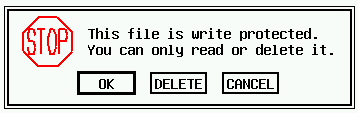
\includegraphics[width=0.5\textwidth]{alert1.eps}
\caption{A message box.}
\label{alert1}
\end{SCfigure}

Fig.~\ref{alert1} shows a typical messagebox. 
The command which produces it is:
\begin{mdframed}[hidealllines=true,backgroundcolor=blue!20]
\begin{verbatim}
ALERT 3,"This file is write protected.|You can only read or \
         delete it.",1,"OK|DELETE|CANCEL",sel
\end{verbatim}
\end{mdframed}

ALERT boxes can also be used to manage simple input forms 
like the one you can see in fig.~\ref{alert3}. 
Here is a little example program:
\begin{mdframed}[hidealllines=true,backgroundcolor=blue!20]
\begin{verbatim}
CLEARW 
i=1
name$="TEST01"
posx$="N54�50'32.3"
posy$="E007�50'32.3"
t$="Edit waypoint:||Name:   "+CHR$(27)+name$+"|"
t$=t$+"Breite: "+chr$(27)+posx$+"|"
t$=t$+"L�nge:  "+chr$(27)+posy$+"|"
t$=t$+"H�he:   "+chr$(27)+str$(alt,5,5)+"|"
t$=t$+"Typ:    "+chr$(27)+hex$(styp,4,4)+"|" 
ALERT 0,t$,1,"OK|UPDATE|L�SCHEN|CANCEL",a,f$
WHILE LEN(f$)
  WORT_SEP f$,CHR$(13),0,a$,f$
  PRINT "Feld";i;": ",a$
  INC i
WEND
QUIT
\end{verbatim}
\end{mdframed}

\begin{SCfigure}
  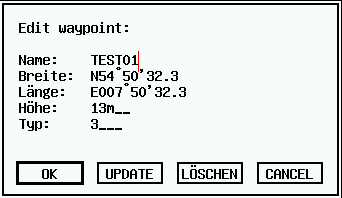
\includegraphics[width=0.5\textwidth]{alert3.eps}
  \caption{A simple input box.}
  \label{alert3}
\end{SCfigure}


\begin{SCfigure}
  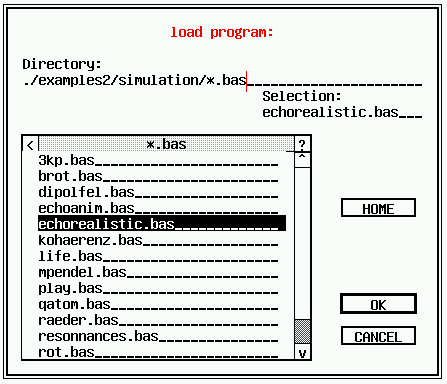
\includegraphics[width=0.7\textwidth]{fileselect.eps}
  \caption{The fileselecetor}
  \label{filesel}
\end{SCfigure}
Fig.~\ref{filesel} shows the fileselector box. The command which produces it is:
\begin{mdframed}[hidealllines=true,backgroundcolor=blue!20]
\begin{verbatim}
FILESELECT "load program:","./*.bas","in.bas",f$
\end{verbatim}
\end{mdframed}

The complete path and filename of the selected file will be returned in 
\verb|f$|.


\begin{SCfigure}
  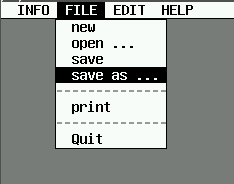
\includegraphics[width=0.3\textwidth]{menu.eps}
  \caption{A pull down menu}
  \label{filesel}
\end{SCfigure}


\section{Resources}

X11-Basic resources consist of object trees, strings, and bitmaps used by a
basic program. They encapsulate the user interface and make internationalization
easier by placing all program strings in a single file. The data format of
X11Basic resource is downwards compatible with the Atari-ST GEM implementation.

\begin{figure}
\begin{center}

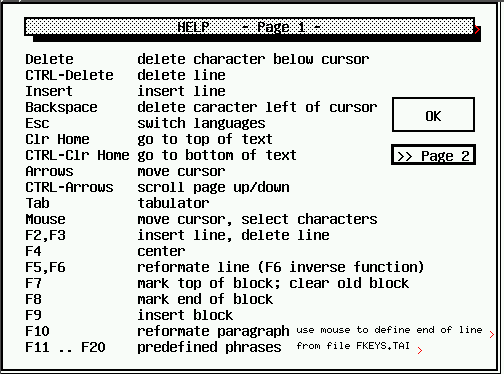
\includegraphics[width=0.48\textwidth]{form1.eps}
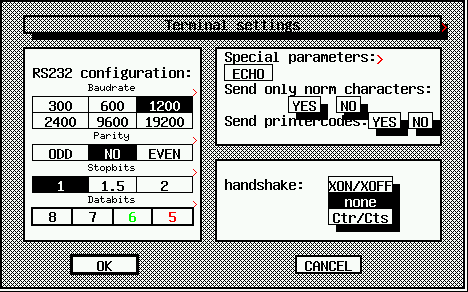
\includegraphics[width=0.48\textwidth]{form2.eps}
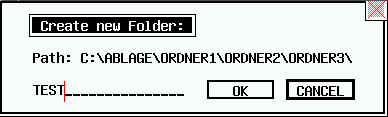
\includegraphics[width=0.48\textwidth]{form3.eps}
\end{center}
\caption{Examples of forms in X11-Basic}
\label{form1}
\end{figure}



Resources are generally created using a Resource Construction
Set (RCS) and saved to a \verb|.RSC| file which is loaded by 
\verb|RSRC_LOAD()| at program initialization time.

Resources may also be embedded as data structures in source code (the 
utility programs \verb|rsc2gui.bas| and \verb|gui2bas.bas| convert \verb|.RSC| files to 
source code). 
Resources contain pointers and coordinates which must be fixed up
before being used.
\verb|RSRC_LOAD()| does this automatically, however if you use an embedded
resource you must take care of this by yourself on each object in each object
tree to convert the initial character coordinates of to screen coordinates.
This allows resources designed on screens with different aspect ratios and
system fonts to appear the same. 
Once a resource is loaded use \verb|rsrc_gaddr()| to obtain pointers to
individual object trees which can then be manipulated directly or with the 
X11-Basic built-in functions. 

\subsection{Objects}

Objects can be boxes, buttons, text, images, and more. An object tree
is an array of OBJECT structures linked to form a structured
relationship to each other. The object itself is a section of data 
which can be held by a string in X11-Basic.

The OBJECT structure is format is as follows:

\begin{verbatim}
object$=MKI$(ob_next)+MKI$(ob_head)+MKI$(ob_tail)+
        MKI$(ob_type)+MKI$(ob_flags)+MKI$(ob_state)+
        MKL$(ob_spec)+MKI$(ob_x)+MKI$(ob_y)+MKI$(ob_width)+
        MKI$(ob_height)
\end{verbatim}

An Object tree is a collection of objects:

\begin{verbatim}
tree$=object0$+object1$+ ... +objectn$
\end{verbatim}

The first object in an OBJECT tree is called the ROOT object (OBJECT 0). It's
coordinates are relative to the upper-left hand corner of the graphics window. 
The ROOT object can have any number of children and each child can have
children of their own. In each case, the OBJECT's coordinates, \verb|ob_x|,
\verb|ob_y|, \verb|ob_width|, and \verb|ob_height| are relative to that of its
parent. The X11-Basic function \verb|objc_offset()| can, however, be used to
determine the exact screen coordinates of a child object. \verb|objc_find()| is
used to determine the object at a given screen coordinate.

The \verb|ob_next|, \verb|ob_head|, and \verb|ob_tail| fields determine this
relationship between parent OBJECTs and child OBJECTs.

\begin{description}

\item[ob\_next] the index (counting objects from the first object in the
object tree) of the object's next sibling at the same level in the object tree
array. The ROOT object should set this value to -1. The last child at any given
nesting level should set this to the index of its parent.

\item[ob\_head] the index of the first child of the current object. If the
object has no children then this value should be -1. 

\item[ob\_tail] the index of the last child: the tail of the list of the
object's children in the object tree array If the object has no children then
this value should be -1.

\item[ob\_type] the object type. The low byte of the ob\_type field 
specifies the object type as follows:

\begin{center}\begin{longtable}{|cll|}
\hline
{\bf ob\_type} & {\bf Name} & {\bf Description}\\
\hline
  20 &  G\_BOX	    &   Box		\\	    
  21 &  G\_TEXT	    &   Formatted Text  \\	    
  22 &  G\_BOXTEXT   &   Formatted Text in a Box \\
  23 &  G\_IMAGE     &   Monochrome Image	\\    
  24 &  G\_PROGDEF   &   Programmer-Defined Object\\
  25 &  G\_IBOX	    &   Invisible Box		  \\  
  26 &  G\_BUTTON    &   Push Button w/String	   \\ 
  27 &  G\_BOXCHAR   &   Character in a Box	   \\ 
  28 &  G\_STRING    &   Un-formatted Text	   \\ 
  29 &  G\_FTEXT     &   Editable Formatted Text \\
  30 &  G\_FBOXTEXT  &   Editable Formatted Text in a Box\\
  31 &  G\_ICON	    &   Monochrome Icon \\
  32 &  G\_TITLE     &   Menu Title\\
  33 &  G\_CICON     &   Color Icon \\
\hline
\end{longtable}\end{center}

\item[ob\_flags] The ob\_flags field of the object structure is a bitmask of
different flags that can be applied to any object. You may want to apply 
one ore more flags at once. Just add the values ob\_flags.

\begin{center}\begin{longtable}{|clp{10cm}|}
\hline
{\bf ob\_flags} & {\bf Name} & {\bf Description}\\
\hline
0 & NONE       & No flag \\\hline
1 & SELECTABLE & object is selected. state may be toggled by clicking on it with the mouse.\\\hline
2 & DEFAULT    & An EXIT object with this bit set will have a thicker outline and be triggered when the 
                 user presses return.\\\hline
4 & EXIT       & Clicking on this OBJECT and releasing the mouse button while still over it 
                 will cause the dialog to exit.\\\hline
8 & EDITABLE   & Set for FTEXT and FBOXTEXT objects to indicate that they may receive edit focus.\\\hline
16 & RBUTTON   & This object is one of a group of radio buttons. Clicking on it will deselect
                 any selected objects at the same tree level that also have the RBUTTON flag
                 set. Likewise, it will be deselected automatically when any other object is selected.\\\hline
32 & LASTOB    & This flag signals that the current OBJECT is the last in the object tree. (Required!)\\\hline
64 & TOUCHEXIT & Setting this flag causes the OBJECT to return an exit state immediately after   
                 being clicked on with the mouse.\\\hline
256 & HIDETREE & This OBJECT and all of its children will not be drawn.\\\hline
512 & INDIRECT & This flag cause the ob\_spec field to be interpreted as a pointer to the      
                 ob\_spec value rather than the value itself.\\\hline
1024 & FL3DIND & Setting this flag causes the OBJECT to be drawn as a 3D indicator. This is  
                 appropriate for radio and toggle buttons.\\\hline
2048 & FL3DACT & Setting this flag causes the OBJECT to be drawn as a 3D activator. This is  
                 appropriate for EXIT buttons.\\\hline
3072 & FL3DBAK & If these bits are set, the object is treated as an AES background object.  
                 If it is OUTLINED, the outlined is drawn in a 3D manner. If its color
                 is set to WHITE and its fill pattern is set to 0 then the OBJECT will inherit 
                 the default 3D background color.\\\hline
4096 & SUBMENU & This bit is set on menu items which have a sub-menu attachment. This bit also
                 indicates that the high byte of the ob\_type field is being used by the menu
                 system.\\\hline
\end{longtable}\end{center}

\item[ob\_state] The ob\_state field determines the display state of the object as
follows:

\begin{center}\begin{longtable}{|clp{10cm}|}
\hline
{\bf ob\_state} & {\bf Name} & {\bf Description}\\
\hline
0 & NORMAL   & Normal state \\\hline
1 & SELECTED & The object is selected. An object with this bit set will be drawn in inverse
               video except for G\_CICON which will use its 'selected' image.\\\hline
2 & CROSSED  & An OBJECT with this bit set will be drawn over with a white cross (this   
               state can only usually be seen over a colored or	SELECTED object).\\\hline
4 & CHECKED  & An OBJECT with this bit set will be displayed with a check mark in its    
               upper-left corner.\\\hline
8 & DISABLED & An OBJECT with this bit set will ignore user input. Text objects with this   
               bit set will draw in grey or a dithered pattern.\\\hline
16 & OUTLINED & G\_BOX, G\_IBOX, G\_BOXTEXT, G\_FBOXTEXT, and G\_BOXCHAR OBJECTs   
               with this bit set will be drawn with a double border.\\\hline
32 & SHADOWED & G\_BOX, G\_IBOX, G\_BOXTEXT, G\_FBOXTEXT, and G\_BOXCHAR OBJECTs   
                will be drawn with a shadow.\\\hline
\end{longtable}\end{center}

\item[ob\_spec] The object-specific field

The ob\_spec field contains different data depending on the object type
as indicated in the table below:
\begin{center}\begin{longtable}{|lp{10cm}|}
\hline
G\_BOX &
The low 16 bits contain a WORD containing color information for the OBJECT. 
Bits 23-16 contain a signed BYTE representing the border thickness of the 
box.\\\hline
G\_TEXT &The ob\_spec field contains a pointer to a TEDINFO  structure. \\\hline  
G\_BOXTEXT &The ob\_spec field contains a pointer to a TEDINFO structure.   \\\hline
G\_IMAGE   & The ob\_spec field points to a BITBLK structure. \\\hline
G\_PROGDEF & The ob\_spec field points to a APPLBLK structure.\\\hline
G\_IBOX	  & The low 16 bits contain a WORD containing color information for the OBJECT. 
Bits 23-16 contain a signed BYTE representing the border thickness of the box.\\\hline
G\_BUTTON  & The ob\_spec field contains a pointer to the text to be contained in the button.\\\hline
G\_BOXCHAR & The low 16 bits contain a WORD containing color information for the OBJECT. 
Bits 23-16 contain a signed BYTE representing the border thickness of the box. 
Bits 31-24 contain the ASCII value of the character to display.\\\hline
G\_STRING  & The ob\_spec field contains a pointer to the text to be displayed.\\\hline
G\_FTEXT   & The ob\_spec field contains a pointer to a TEDINFO structure.\\\hline
G\_FBOXTEXT & The ob\_spec field contains a pointer to a TEDINFO structure.\\\hline
G\_ICON & The ob\_spec field contains a pointer to an ICONBLK structure. \\\hline    
G\_TITLE  & The ob\_spec field contains a pointer to the text to be used for the title.\\\hline
G\_CICON  & The ob\_spec field contains a pointer to a CICONBLK structure.\\\hline
\end{longtable}\end{center}

\begin{description}
\item[objc\_colorword]
Almost all objects reference a WORD containing the object color as
defined below.

\begin{verbatim}
objc_colorword=bbbbcccctpppcccc

Bits 15-12 contain the border color 
Bits 11-8  contain the text color 
Bit   7    is 1 if opaque or 0 if transparent 
Bits 6-4   contain the fill pattern index 
Bits 3-0   contain the fill color 
\end{verbatim}

Available colors for fill patterns, text, and borders are listed
below:
\begin{center}
\begin{tabular}{|cll|}
\hline
{\bf Value} &{\bf  Name}&{\bf  Color}  \\
\hline
 0&  WHITE	&  White\\
 1&  BLACK	&  Black\\
 2&  RED	&  Red\\
 3&  GREEN	&  Green\\
 4&  BLUE	&  Blue\\
 5&  CYAN	&  Cyan\\
 6&  YELLOW	&  Yellow\\
 7&  MAGENTA	&  Magenta\\
 8&  LWHITE	&  Light Gray\\
 9&  LBLACK	&  Dark Gray\\
 10& LRED	&  Light Red\\
 11& LGREEN	&  Light Green\\
 12& LBLUE	&  Light Blue\\
 13& LCYAN	&  Light Cyan\\
 14& LYELLOW	&  Light Yellow\\
 15& LMAGENTA	&  Light Magenta\\
\hline
\end{tabular}
\end{center}


\item[TEDINFO]
G\_TEXT, G\_BOXTEXT, G\_FTEXT, and G\_FBOXTEXT objects all reference a
TEDINFO structure in their ob\_spec field. The TEDINFO structure is
defined below:
 {\footnotesize
\begin{verbatim}                                                         
tedinfo$=MKL$(VARPTR(te_ptext$))+MKL$(VARPTR(te_ptmplt$))+
         MKL$(VARPTR(te_pvalid$))+MKI$(te_font)+MKI$(te_fontid)+
         MKI$(te_just)+MKI$(te_color)+MKI$(te_fontsize)+
         MKI$(te_thickness)+MKI$(te_txtlen)+MKI$(te_tmplen)
\end{verbatim}}

The three character pointers point to text strings required for 
\verb|G_FTEXT|
and \verb|G_FBOXTEXT| objects. te\_ptext points to the actual text to be
displayed and is the only field used by all text objects. te\_ptmplt
points to the text template for editable fields. For each character
that the user can enter, the text string should contain a tilde
character (ASCII 126). Other characters are displayed but cannot be
overwritten by the user. \verb|te_pvalid| contains validation characters for
each character the user may enter. The current acceptable validation
characters are:

\begin{tabbing}
XXXXX\=XXXXXXXXXXXX\=\kill\\
{\bf Char} \> {\bf  Allows}\\
9 \> Digits 0-9\\
A \> Uppercase letters A-Z plus space\\
a \> Upper and lowercase letters plus space\\
N \> Digits 0-9, uppercase letters A-Z and space\\
n \> Digits 0-9, upper and lowercase letters A-Z  and space\\
F \> Valid DOS filename characters plus question mark and asterisk \\
P \> Valid DOS pathname characters, backslash, colon, \\
  \> question mark, asterisk \\
p \> Valid DOS pathname characters, backslash and colon\\
X \> All characters\\
\end{tabbing}

\verb|te_font| may be set to any of the following values:

\begin{center}
\begin{tabular}{|cll|}
\hline
{\bf te\_font} &{\bf  Name} & {\bf Description} \\
\hline
3 &IBM    & Use the standard monospaced font.\\
5 &SMALL  &  Use the small monospaced font.\\
\hline
\end{tabular}
\end{center}

\verb|te_just| sets the justification of the text output as follows:

\begin{center}
\begin{tabular}{|cll|}
\hline
{\bf te\_just} &{\bf  Name} & {\bf Description} \\
\hline
0 & TE\_LEFT & Left Justify\\
1 & TE\_RIGHT & Right Justify\\
2 & TE\_CNTR & Center\\
\hline
\end{tabular}
\end{center}


te\_thickness sets the border thickness (positive and negative values
are acceptable) of the G\_BOXTEXT or G\_FBOXTEXT object. 

te\_txtlen and
te\_tmplen should be set to the length of the starting text and
template length respectively. 

\item[BITBLK]
G\_IMAGE objects contain a pointer to a BITBLK structure in their
ob\_spec field. The BITBLK structure is defined as follows:

 {\footnotesize
\begin{verbatim}                                                         
bitblk$=MKL$(VARPTR(bi_pdata$))+MKI$(bi_wb)+MKI$(bi_hl)+
        MKI$(bi_x)+MKI$(bi_y)+MKI$(bi_color)
\end{verbatim}}

\verb|bi_pdata| should contain a monochrome bit image. 
\verb|bi_wb| specifies the width (in bytes) of the image. 
All BITBLK images must be a multiple of 16 pixels wide therefore this 
value must be even.
\verb|bi_hl| specifies the height of the image in scan lines (rows). 
\verb|bi_x| and \verb|bi_y| are used as offsets into \verb|bi_pdata|. 
Any data occurring before these coordinates will be ignored. 
\verb|bi_color| is a standard color WORD
where the fill color specifies the color in which the image will be
rendered.

\item[ICONBLK]
The \verb|ob_spec| field of \verb|G_ICON| objects point to an ICONBLK structure as
defined below:

 {\footnotesize
\begin{verbatim}                                                         
iconblk$=MKL$(VARPTR(ib_pmask$))+MKL$(VARPTR(ib_pdata$))+MKL$(VARPTR(ib_ptext$))+
         MKI$(ib_char)+MKI$(ib_xchar)+MKI$(ib_ychar)+
         MKI$(ib_xicon)+MKI$(ib_yicon)+MKI$(ib_wicon)+MKI$(ib_hicon)+
	 MKI$(ib_xtext)+MKI$(ib_ytext)+MKI$(ib_wtext)+MKI$(ib_htext)
\end{verbatim}}

\verb|ib_pmask| and \verb|ib_pdata| contain the monochrome mask and 
image data respectively. \verb|ib_ptext| is a string pointer to the icon text.
\verb|ib_char| defines the icon character (used for drive icons) and the icon
foreground and background color as follows:

 {\footnotesize
\begin{verbatim}                                                         
|                              ib_char                               |
|      Bits 15-12      |      Bits 11-8       |       Bits 7-0       |
|Icon Foreground Color |Icon Background Color |ASCII Character (or 0 |
|                      |                      |  for no character).  |
\end{verbatim}}

\verb|ib_xchar| and \verb|ib_ychar| specify the location of the icon character
relative to \verb|ib_xicon| and \verb|ib_yicon|. \verb|ib_xicon| and 
\verb|ib_yicon| specify the
location of the icon relative to the \verb|ob_x| and \verb|ob_y| of the object.
\verb|ib_wicon| and \verb|ib_hicon| specify the width and height of the icon in
pixels. As with images, icons must be a multiple of 16 pixels in
width.
\verb|ib_xtext| and \verb|ib_ytext| specify the location of the text string relative
to the \verb|ob_x| and \verb|ob_y| of the object. \verb|ib_wtext| and \verb|ib_htext| specify the
width and height of the icon text area.

\item[CICONBLK]

The \verb|G_CICON| object defines its
\verb|ob_spec| field to be a pointer to a CICONBLK structure as defined
below:

 {\footnotesize
\begin{verbatim}                                                         
ciconblk$=monoblk$+MKL$(VARPTR(mainlist$))
\end{verbatim}}

\verb|monoblk| contains a monochrome icon which is rendered if a color icon
matching the display parameters cannot be found. In addition, the icon
text, character, size, and positioning data from the monochrome icon
are always used for the color one. \verb|mainlist| contains the first
CICON structure in a linked list of color icons for different
resolutions. \verb|CICON| is defined as follows:

 {\footnotesize
\begin{verbatim}                                                         
cicon$=MKI$(num_planes)+MKL$(VARPTR(col_data$))+MKL$(VARPTR(col_mask$))+
       MKL$(VARPTR(sel_data$))+MKL$(VARPTR(sel_mask$))+
       MKL$(VARPTR(cicon2$))
\end{verbatim}}

\verb|num_planes| indicates the number of bit planes this color icon
contains. \verb|col_data| and \verb|col_mask| contain the icon data and 
mask for the unselected icon respectively. Likewise, 
\verb|sel_data| and \verb|sel_mask| contain the icon data and mask for 
the selected icon. \verb|cicon2$| contains
the next color icon definition. Use \verb|MKL$(0)| if no more are available.

The GUI library searches the CICONBLK object for a color icon that has the
same number of planes in the display. If none is found, the GUI library simply
uses the monochrome icon.

\item[APPLBLK]

\verb|G_PROGDEF| objects allow programmers to define custom objects and link
them transparently in the resource. The \verb|ob_spec| field of
\verb|G_PROGDEF|
objects contains a pointer to an APPLBLK as defined below:

 {\footnotesize
\begin{verbatim}                                                         
applblk$=MKL$(SYM_ADR(#1,"function"))+MKL$(ap_parm)
\end{verbatim}}

The first is a pointer to a user-defined routine which will draw the
object. This routine must be a c-Function, which has to be linked to 
X11-basic with the LINK command. The routine will be passed a pointer to a
PARMBLK structure containing the information it needs to render the
object. The routine must be defined with stack checking off and expect
to be passed its parameter on the stack. \verb|ap_parm| is a user-defined
value which is copied into the PARMBLK structure as defined below:

{\footnotesize
\begin{verbatim}                                                         
typedef struct parm_blk {
        OBJECT          *tree;
        short            pb_obj;
        short            pb_prevstate;
        short            pb_currstate;
        short            pb_x;
        short            pb_y;
        short            pb_w;
        short            pb_h;
        short            pb_xc;
        short            pb_yc;
        short            pb_wc;
        short            pb_hc;
        long             pb_parm;
} PARMBLK;
\end{verbatim}}

\verb|tree| points to the OBJECT tree of the object being drawn. The object
is located at index \verb|pb_obj|.

The routine is passed the old \verb|ob_state| of the object in
\verb|pb_prevstate|
and the new \verb|ob_state| of the object in \verb|pb_currstate|. 
If \verb|pb_prevstate|
and \verb|pb_currstate| is equal then the object should be drawn completely,
otherwise only the drawing necessary to redraw the object from
\verb|pb_prevstate| to \verb|pb_currstate| are necessary.

\verb|pb_x|, \verb|pb_y|, \verb|pb_w|, and \verb|pb_h| give the screen 
coordinates of the object.
\verb|pb_xc|, \verb|pb_yc|, \verb|pb_wc|, and \verb|pb_hc| give the 
rectangle to clip to. \verb|pb_parm|
contains a copy of the \verb|ap_parm| value in the APPLBLK structure.
The custom routine should return a short containing any remaining
\verb|ob_state| bits you wish the GUI Library to draw over your custom object.

\end{description}

\end{description}



\subsubsection{Dialogs}

Dialog boxes are modal forms of user input. This means that no other
interaction can occur between the user and applications until the
requirements of the dialog have been met and it is exited. A normal
dialog box consists of an object tree with a BOX
as its root object and any number of other controls that accept user
input. Both alert boxes and the file selector are examples of
dialog boxes.

The \verb|form_do()| function performs the simplest method of using a dialog box. Simply
construct an OBJECT tree with at least one EXIT or TOUCHEXIT object and call
\verb|form_do()|\footnote{Before you should display the dialog box using the
{\tt objc\_draw()} function. Maybe you also want to center the dialog with 
{\tt form\_center()} and save and redraw the background 
with {\tt form\_dial()}.}. All interaction with the dialog like editable fields,
radio buttons, and selectable objects will be maintained by the 
X11-Basic library until the
user strikes an EXIT or TOUCHEXIT object.


\subsection{The gui file format}

The *.gui file format, which is basically an ASCII representation of the ATARI
ST resource files (*.rsc), can be converted to X11-Basic code, which then can
handle message boxes and forms. The converter \verb|gui2bas(1)| does this job.
For conversion of ATARI ST resource files to *.gui Files see \verb|rsc2gui(1)|.

The *.gui file consists of Lines and Blocks which specify objects and their 
hierarchical dependencies.
The generic format of such an object is:

\begin{verbatim}
label: TYPE(variables) {
 ... block ...
}
\end{verbatim}

The label is optional and gives the object a name. Depending on TYPE of the
object, one or more variables are given as a comma separated list in
brackets. 

Each object may start a block with '\{' at the end of the line. Inside this
block there might be one or more objects given which then are considered as
sub-objects of the one which opened the block. The block will be closed by a
'\}' in a single line.

\begin{mdframed}[hidealllines=true,backgroundcolor=green!20]

Example:

{\footnotesize\linespread{0.8}
\begin{verbatim}
' Little selector box  (c) Markus Hoffmann    07.2003
' convert this with gui2bas !
' as an example for the use of the gui system
' with X11-Basic

BOX(X=0,Y=0,W=74,H=14, FRAME=2, FRAMECOL=1, TEXTCOL=1, BGCOL=0, PATTERN=0, TEXTMODE=0, 
    STATE=OUTLINED+) {
  BOXTEXT(X=2,Y=1,W=70,H=1, TEXT="Select option ...", FONT=3, JUST=2, COLOR=4513, 
          BORDER=253, STATE=SHADOWED+)
  BOX(X=2,Y=3,W=60,H=10, FRAME=-1, FRAMECOL=1, TEXTCOL=1, BGCOL=0, PATTERN=0, 
      TEXTMODE=0) {
    FTEXT(X=1,Y=1,W=30,H=1,COLOR=4513,FONT=3,BORDER=1,TEXT="Line 1", 
          PTMP="_______________________________________",
          PVALID="XXXXXXXXXXXXXXXXXXXXXXXXXXXXXXXXXXXXXXX", FLAGS=EDITABLE)
    FTEXT(X=1,Y=2,W=30,H=1,COLOR=4513,FONT=3,BORDER=1,TEXT="", 
          PTMP="_______________________________________",
          PVALID="XXXXXXXXXXXXXXXXXXXXXXXXXXXXXXXXXXXXXXX", FLAGS=EDITABLE)
    FTEXT(X=1,Y=3,W=30,H=1,COLOR=4513,FONT=3,BORDER=1,TEXT="", 
          PTMP="_______________________________________",
          PVALID="XXXXXXXXXXXXXXXXXXXXXXXXXXXXXXXXXXXXXXX", FLAGS=EDITABLE)
    FTEXT(X=1,Y=4,W=30,H=1,COLOR=4513,FONT=3,BORDER=1,TEXT="", 
          PTMP="_______________________________________",
          PVALID="XXXXXXXXXXXXXXXXXXXXXXXXXXXXXXXXXXXXXXX", FLAGS=EDITABLE)
    BOX(X=2,Y=6,W=50,H=3, FRAME=-1, FRAMECOL=1, TEXTCOL=1, BGCOL=1, PATTERN=5, 
          TEXTMODE=0) { 
      BUTTON(X=2,Y=1,W=4,H=1, TEXT="ON",STATE=SELECTED, 
             FLAGS=RADIOBUTTON+SELECTABLE,FRAME=2, FRAMECOL=1, TEXTCOL=1, 
             BGCOL=1, PATTERN=0, TEXTMODE=0)
      BUTTON(X=8,Y=1,W=4,H=1, TEXT="OFF",FLAGS=RADIOBUTTON+SELECTABLE,FRAME=2, 
             FRAMECOL=1, TEXTCOL=1, BGCOL=1, PATTERN=0, TEXTMODE=0)
    }
  }
  ok:	  BUTTON(X=65,Y=4,W=7,H=4, TEXT="OK", FLAGS=SELECTABLE+DEFAULT+EXIT)
  cancel: BUTTON(X=65,Y=9,W=7,H=4, TEXT="CANCEL", FLAGS=SELECTABLE+EXIT+LASTOB+)
}
\end{verbatim}
}
\end{mdframed}

\section{Menus}

Most applications use a menu bar to allow the user to navigate through program
options.

Here is a simple example program, which demonstrates the handling of a drop
down menu. 

\begin{mdframed}[hidealllines=true,backgroundcolor=blue!20]
{\footnotesize\linespread{0.8}
\begin{verbatim}
' Test-program for Drop-Down-Menus
'
DIM field$(50)
FOR i=0 TO 50
  READ field$(i)
  EXIT IF field$(i)="***"
NEXT i
oh=0
field$(i)=""
DATA "INFO","  Menutest"
DATA "---------------"
DATA "- Access.1","- Access.2","- Access.3","- Access.4","- Access.5"
DATA "- Access.6",""
DATA "FILE","  new","  open ...","  save","  save as ...","--------------"
DATA "  print","--------------","  Quit",""
DATA "EDIT","  cut","  copy","  paste","----------","  help1","  helper"
DATA "  assist",""
DATA "HELP","  online help","--------------","  edifac","  editor","  edilink"
DATA "  edouard",""
DATA "***"

grau=GET_COLOR(32000,32000,32000)
COLOR grau
PBOX 0,0,640,400
MENUDEF field$(),menuaction
DO 
  PAUSE 0.05
  MENU 
LOOP
QUIT

PROCEDURE menuaction(k)
  LOCAL b
  IF (field$(k)="  Quit") OR (field$(k)="  exit") 
    QUIT
  ELSE IF field$(k)="  online help"
    oh=not oh
    MENUSET k,4*abs(oh)
  ELSE IF field$(k)="  Menutest" 
    ~FORM_ALERT(1,"[0][- Menutest -||(c) Markus Hoffmann 2001|X11-Basic V.1.03][ OK ]")
  ELSE   
    PRINT "MENU selected ";k;" contents: ";field$(k)
    b=FORM_ALERT(1,"[1][--- Menutest ---||You selected item (No. "+str$(k)+ \
                   "),| for which was no|function defined !][ OK |disable]")
    IF b=2
      MENUSET k,8
    ENDIF
  ENDIF
RETURN
\end{verbatim}
}
\end{mdframed}
